
%%%%%%%%%%%%%%%%%%%%%%%%%%%%%%%%%%%%%%%%%%
%%                                      %%
%%          Resultados Obtidos          %%
%%                                      %%
%%%%%%%%%%%%%%%%%%%%%%%%%%%%%%%%%%%%%%%%%%

% Neste capítulo são expostos os resultados de sua pesquisa. 
% No caso do TCC I, resultados esperados ou parciais, para TCC II, resultados "finais".

\chapter{Resultados}
    \label{cha:resultados}
    Neste capítulo são discutidos os resultados obtidos após a aplicação da proposta apresentada no Capítulo~\ref{cha:desenvolvimento-da-pesquisa}.
    A abordagem possui dois momentos: no primeiro momento, descrito na Seção~\ref{sec:effectiveness-analysis}, são apresentados os resultados obtidos por cada classificador individualmente, além de análises do parâmetro $cr$ por classificador e por cada variação do método \ac{flexcon}; no segundo momento, Seção~\ref{sec:statistical-analysis}, é conduzida uma análise estatística dos resultados obtidos.

    % Pegar dados do Planilhas do Google Drive e transforma-los em gráficos de linhas onde o eixo X representa a porcentagem de inicialmente rotulados, o Y a porcentagem da acurácia do método e a linha representa a porcentagem de variação do limiar

    % Como resultados parciais deste trabalho destacam\hyp{se} a aplicação de três taxas de variações (3\%, 5\% e 7\%) que manipulam o limiar da iteração seguinte. O método \textit{FlexCon\hyp{C1} (v)} foi aplicado a um conjunto de três bases de dados (\textit{Mammographic Mass}, \textit{Mfeat\hyp{karhunen}} e \textit{Mushroom}). A Tabela~\ref{tab:partial-results} apresenta as acurácias obtidas para cada uma das bases de dados utilizando o método \textit{FlexCon\hyp{C1} (v)} aliado ao classificador Naive Bayes.

    % \begin{table}[h]
    %     \centering
    %     \caption{Acurácia do \textit{FlexCon\hyp{C1} (v)} utilizando o classificador Naive Bayes.}
    %     \label{tab:partial-results}
    %     \resizebox{\textwidth}{!}{%
    %         \begin{tabular}{|c|c|c|c|c|c|c|}
    %             \toprule
    %             \multirow{2}{*}{\textbf{Base de Dados}}     & \multirow{2}{*}{\textbf{Taxa de Variação}} & \multicolumn{5}{c|}{\textbf{Inicialmente Rotulados}} \\ \cmidrule(l){3-7} 
    %                                               &                                   & \textbf{5\%}     & \textbf{10\%}   & \textbf{15\%}   & \textbf{20\%}   & \textbf{25\%}   \\ \midrule
    %             \multirow{3}{*}{Mammographic Mass} & 3\%                               & 75.83\%   & 75.42\%  & 77.08\%  & 75.83\%  & 77.92\%  \\ \cmidrule(l){2-7} 
    %                                               & 5\%                               & 75.83\%   & 75.42\%  & 77.08\%  & \textbf{76.25\%}  & 77.92\%  \\ \cmidrule(l){2-7} 
    %                                               & 7\%                               & 75.83\%   & 75.42\%  & 77.08\%  & 75.83\%  & 77.92\%  \\ \midrule
    %             \multirow{3}{*}{Mfeat\hyp{karhunen}}    & 3\%                               & 84.60\%   & 88.00\%  & 90.20\%  & \textbf{90.60\%}  & 89.40\%  \\ \cmidrule(l){2-7} 
    %                                               & 5\%                               & \textbf{85.40\%}   & \textbf{88.60\%}  & \textbf{91.20\%}  & \textbf{90.60\%}  & \textbf{90.00\%}  \\ \cmidrule(l){2-7} 
    %                                               & 7\%                               & 84.60\%   & 88.00\%  & 90.20\%  & 90.40\%  & 89.40\%  \\ \midrule
    %              \multirow{3}{*}{Mushroom}          & 3\%                               & 89.66\%   & 90.89\%  & 91.68\%  & 90.65\%  & \textbf{93.11\%}  \\ \cmidrule(l){2-7} 
    %                                               & 5\%                               & \textbf{90.74\%}   & \textbf{92.12\%}  & \textbf{92.27\%}  & \textbf{91.97\%}  & 92.61\%  \\ \cmidrule(l){2-7} 
    %                                               & 7\%                               & 89.66\%   & 90.50\%  & 91.19\%  & 91.04\%  & 91.29\%  \\ \bottomrule
    %         \end{tabular}
    %     }
    %     \source{O Próprio Autor (\imprimirdata)}
    % \end{table}

    % As Figuras~\ref{fig:base-mammographic}, \ref{fig:base-mfeat-karhunen} e \ref{fig:base-mushroom} apresentam gráficos sintetizando as informações contidas na Tabela~\ref{tab:partial-results} para as bases de dados \textit{Mammographic Mass}, \textit{Mfeat\hyp{karhunen}} e \textit{Mushroom} respectivamente. Nestes gráficos estão representados os percentuais de exemplos inicialmente rotulados pelas acurácias obtidas alterando a taxa de variação do limiar.

    % \begin{figure}[h]
    %     \centering
    %     \caption{Percentuais de Exemplos Inicialmente Rotulados x Acurácia Obtida na Base \textit{Mammographic Mass}.}
    %     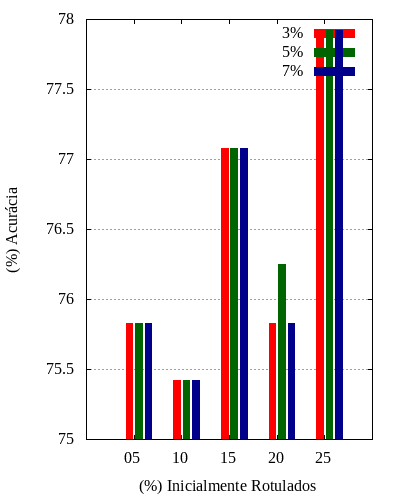
\includegraphics[scale=0.5]{figuras/Mammographic.png}
    %     \label{fig:base-mammographic}
    %     \source{O Próprio Autor (\imprimirdata)}
    % \end{figure}

    % \begin{figure}[h]
    %     \centering
    %     \caption{Percentuais de Exemplos Inicialmente Rotulados x Acurácia Obtida na Base \textit{Mfeat\hyp{karhunen}}.}
    %     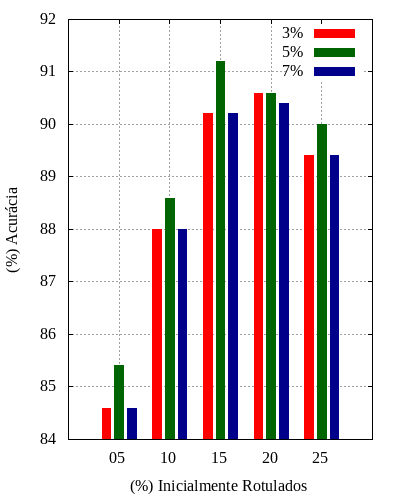
\includegraphics[scale=0.5]{figuras/Mfeat-karhunen.png}
    %     \label{fig:base-mfeat-karhunen}
    %     \source{O Próprio Autor (\imprimirdata)}
    % \end{figure}

    % \begin{figure}[h]
    %     \centering
    %     \caption{Percentuais de Exemplos Inicialmente Rotulados x Acurácia Obtida na Base \textit{Mushroom}.}
    %     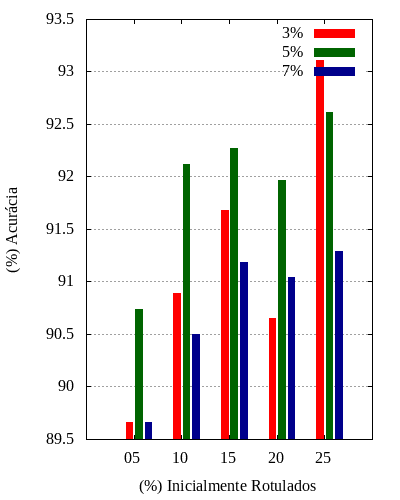
\includegraphics[scale=0.5]{figuras/Mushroom.png}
    %     \label{fig:base-mushroom}
    %     \source{O Próprio Autor (\imprimirdata)}
    % \end{figure}

    % As Tabelas~\ref{tab:naive-acc}-\ref{tab:knn-acc} apresentam em cada uma das células as acurácias médias obtidas pelos classificadores, além de apresentar também o desvio padrão obtido por cada classificador (Na\"ive Bayes, \textit{rpartXse}, \ac{ripper} e \ac{knn}), respectivamente. Em cada uma das referidas tabelas, está sendo analisado a variação do parâmetro $cr$ em diferentes métodos e diferentes percentuais de exemplos rotulados.
    \section{Análise de Eficácia}
        \label{sec:effectiveness-analysis}

        As Tabelas~\ref{tab:naive-acc}-\ref{tab:knn-acc} apresentam os desempenhos obtidas pelo método \ac{flexcon}, considerando\hyp{se} cada uma das técnicas abordadas, \textit{FlexCon\hyp{C1} (s)}, \textit{FlexCon\hyp{C1} (v)} e \textit{FlexCon\hyp{C2}}. Nestas tabelas, as colunas são as variações aplicadas ao parâmetro $cr$, as células apresentam as acurácias médias e o desvio padrão associado obtidas pelos classificadores. Em cada uma das referidas tabelas, estão sendo analisadas as variações do parâmetro $cr$ para diferentes técnicas, diferentes percentuais de exemplos rotulados e, destacado em negrito, a maior acurácia obtida pela respectiva técnica para cada percentual de exemplos inicialmente rotulados. Informações dos resultados para cada técnica e classificador avaliados nos experimentos são apresentadas no Apêndice~\ref{apen:all-results}.
        
        A Tabela~\ref{tab:naive-acc} apresenta os resultados obtidos após a aplicação do classificador Na\"ive Bayes. Os melhores resultados encontram\hyp{se} entre 3\% e 7\% para todas as técnicas analisadas. Realizando uma análise mais detalhada, observa\hyp{se} que os melhores valores estão bastante dispersos, entretanto, para valores intermediários de exemplos inicialmente rotulados recomenda\hyp{se} pré\hyp{fixar} o parâmetro $cr$ entre 3\% e 5\%. De maneira geral, quando o valor do parâmetro $cr$ é pré\hyp{fixado} entre 3\% e 7\% os resultados são distribuídos de forma igualitária, onde cada valor é superior em 3 dos 15 casos, representando 20\% para cada um dos casos. Além disto, o classificador em questão, obteve os mesmos percentuais de acerto quando aplicada às demais técnicas.
    
    \begin{table}[!ht]
        \centering
        \caption{Resultado da acurácia com o classificador Na\"ive Bayes}
        \resizebox{\textwidth}{!} & \textbf{3\%} & \textbf{4\%} & \textbf{5\%} & \textbf{6\%} & \textbf{7\%} & \textbf{8\%} \\ \hline
                \parbox[t]{3mm}{\multirow{5}{*}{\rotatebox[origin=c]{90}{FlexCon-C1(s)}}}
                 & 05\% & $72,38 \pm 18,19$ & $73,19 \pm 17,53$ & $72,59 \pm 17,70$ & $73,10 \pm 17,43$ & $72,85 \pm 17,85$ & $\textbf{73,26} \pm 17,42$ & $73,03 \pm 17,86$ \\
                 & 10\% & $73,71 \pm 16,84$ & $73,16 \pm 17,02$ & $\textbf{74,35} \pm 16,81$ & $73,60 \pm 17,54$ & $72,89 \pm 16,73$ & $73,85 \pm 17,33$ & $73,73 \pm 17,02$ \\
                 & 15\% & $73,23 \pm 17,66$ & $\textbf{73,70} \pm 17,41$ & $73,35 \pm 17,55$ & $73,40 \pm 17,68$ & $73,47 \pm 17,57$ & $72,96 \pm 17,96$ & $73,41 \pm 17,34$ \\
                 & 20\% & $73,24 \pm 17,41$ & $73,49 \pm 17,07$ & $72,98 \pm 17,52$ & $\textbf{74,02} \pm 16,96$ & $73,99 \pm 16,32$ & $73,80 \pm 17,52$ & $73,65 \pm 17,29$ \\
                 & 25\% & $73,68 \pm 17,33$ & $73,74 \pm 17,00$ & $73,89 \pm 17,06$ & $73,47 \pm 17,34$ & $\textbf{74,11} \pm 16,88$ & $73,51 \pm 17,47$ & $73,38 \pm 17,26$ \\ \hline
                \parbox[t]{3mm}{\multirow{5}{*}{\rotatebox[origin=c]{90}{FlexCon-C1(v)}}}
                 & 05\% & $72,38 \pm 18,19$ & $73,19 \pm 17,53$ & $72,59 \pm 17,70$ & $73,10 \pm 17,43$ & $72,85 \pm 17,85$ & $\textbf{73,26} \pm 17,42$ & $73,03 \pm 17,86$ \\
                 & 10\% & $73,71 \pm 16,84$ & $73,16 \pm 17,02$ & $\textbf{74,35} \pm 16,81$ & $73,60 \pm 17,54$ & $72,89 \pm 16,73$ & $73,85 \pm 17,33$ & $73,73 \pm 17,02$ \\
                 & 15\% & $73,23 \pm 17,66$ & $\textbf{73,70} \pm 17,41$ & $73,35 \pm 17,55$ & $73,40 \pm 17,68$ & $73,47 \pm 17,57$ & $72,96 \pm 17,96$ & $73,41 \pm 17,34$ \\
                 & 20\% & $73,24 \pm 17,41$ & $73,49 \pm 17,07$ & $72,98 \pm 17,52$ & $\textbf{74,02} \pm 16,96$ & $73,99 \pm 16,32$ & $73,80 \pm 17,52$ & $73,65 \pm 17,29$ \\
                 & 25\% & $73,68 \pm 17,33$ & $73,74 \pm 17,00$ & $73,89 \pm 17,06$ & $73,47 \pm 17,34$ & $\textbf{74,11} \pm 16,88$ & $73,51 \pm 17,47$ & $73,38 \pm 17,26$ \\ \hline
                \parbox[t]{3mm}{\multirow{5}{*}{\rotatebox[origin=c]{90}{FlexCon-C2}}}
                 & 05\% & $72,38 \pm 18,19$ & $73,19 \pm 17,53$ & $72,59 \pm 17,70$ & $73,10 \pm 17,43$ & $72,85 \pm 17,85$ & $\textbf{73,26} \pm 17,42$ & $73,03 \pm 17,86$ \\
                 & 10\% & $73,71 \pm 16,84$ & $73,16 \pm 17,02$ & $\textbf{74,35} \pm 16,81$ & $73,60 \pm 17,54$ & $72,89 \pm 16,73$ & $73,85 \pm 17,33$ & $73,73 \pm 17,02$ \\
                 & 15\% & $73,23 \pm 17,66$ & $\textbf{73,70} \pm 17,41$ & $73,35 \pm 17,55$ & $73,40 \pm 17,68$ & $73,47 \pm 17,57$ & $72,96 \pm 17,96$ & $73,41 \pm 17,34$ \\
                 & 20\% & $73,24 \pm 17,41$ & $73,49 \pm 17,07$ & $72,98 \pm 17,52$ & $\textbf{74,02} \pm 16,96$ & $73,99 \pm 16,32$ & $73,80 \pm 17,52$ & $73,65 \pm 17,29$ \\
                 & 25\% & $73,68 \pm 17,33$ & $73,74 \pm 17,00$ & $73,89 \pm 17,06$ & $73,47 \pm 17,34$ & $\textbf{74,11} \pm 16,88$ & $73,51 \pm 17,47$ & $73,38 \pm 17,26$ \\ \hline
            \end{tabular}%
        }
        \label{tab:naive-acc}
        \source{O Próprio Autor (\the\year)}
    \end{table}
    
    A Tabela~\ref{tab:rpart-acc} apresenta os resultados obtidos pelo classificador \textit{rpartXse}. Para a técnica \textit{FlexCon\hyp{C1} (s)} observou\hyp{se} melhores resultados ao utilizar valores mais elevados(acima de 5\%) para o parâmetro $cr$, pois no geral apresentam resultados mais significativos em 3 dos 5 percentuais de exemplos considerados. Por sua vez, a técnica \textit{FlexCon\hyp{C1} (v)} obtém resultados mais significativos quando o parâmetro $cr$ é pré\hyp{fixado} entre 5\% e 8\% e, em geral, quando o valor é prefixado em 6\% obtém resultados mais significativos em 2 dos 5 casos. Na técnica \textit{FlexCon\hyp{C2}} o valor de 5\% utilizado no trabalho original obtém os melhores resultados em 2 dos 5 casos. Entretanto, para essa combinação de classificador e técnica os resultados obtidos estão bastante dispersos, parte dos melhores valores concentram\hyp{se} na faixa intermediária 4\% e 5\%, e o restante se divide entre 2\% e 8\% {--} 1 caso para cada. Em geral, observando\hyp{se} todas as combinações classificador e técnica, os melhores resultados tendem para valores iguais ou superiores a 5\%.
    
    % Para o método \textit{FlexCon\hyp{C1} (s)} os melhores valores para o parâmetro $cr$ concentram\hyp{se} em 4\% e 8\% quando pré\hyp{fixa} o parâmetro $cr$ nestes valores os resultados são superiores em 2 dos 5 casos, para ambos valores. O método \textit{FlexCon\hyp{C1} (v)} a valor que se destaca em relação aos demais é o valor de 8\% sendo superior em 2 dos 5 casos. Por sua vez, no método \textit{FlexCon\hyp{C2}} dois valores obtém resultados superiores são eles 5\% e 8\% em 2 dos 5 casos. Observando de maneira geral, os valores de 8\% e 5\% se destacam sendo superiores em 6 dos 15 e 4 dos 15 casos, respectivamente.
    
    \begin{table}[h]
        \centering
        \caption{Resultado da acurácia com o classificador \textit{rpartXse}}
        \resizebox{\textwidth}{!} & \textbf{3\%} & \textbf{4\%} & \textbf{5\%} & \textbf{6\%} & \textbf{7\%} & \textbf{8\%} \\ \hline
                \parbox[t]{3mm}{\multirow{5}{*}{\rotatebox[origin=c]{90}{FlexCon-C1(s)}}}
                 & 05\% & $\textbf{76,17} \pm 14,75$ & $75,58 \pm 15,32$ & $75,49 \pm 15,61$ & $75,23 \pm 16,12$ & $75,92 \pm 15,01$ & $75,45 \pm 15,91$ & $75,67 \pm 15,64$ \\
                 & 10\% & $75,73 \pm 15,72$ & $75,87 \pm 15,50$ & $75,25 \pm 15,82$ & $76,11 \pm 15,25$ & $\textbf{76,18} \pm 15,43$ & $75,64 \pm 15,39$ & $76,00 \pm 15,15$ \\
                 & 15\% & $75,77 \pm 15,41$ & $75,71 \pm 15,48$ & $75,47 \pm 15,71$ & $75,31 \pm 15,79$ & $75,60 \pm 15,90$ & $75,95 \pm 15,28$ & $\textbf{76,06} \pm 15,29$ \\
                 & 20\% & $75,73 \pm 15,44$ & $75,81 \pm 15,39$ & $\textbf{75,99} \pm 15,26$ & $75,80 \pm 15,27$ & $75,89 \pm 15,39$ & $75,66 \pm 15,22$ & $75,91 \pm 14,93$ \\
                 & 25\% & $75,75 \pm 15,36$ & $75,49 \pm 15,21$ & $75,98 \pm 15,24$ & $75,84 \pm 15,20$ & $75,47 \pm 15,29$ & $\textbf{76,00} \pm 15,15$ & $75,15 \pm 15,65$ \\ \hline
                \parbox[t]{3mm}{\multirow{5}{*}{\rotatebox[origin=c]{90}{FlexCon-C1(v)}}}
                 & 05\% & $76,10 \pm 14,73$ & $75,47 \pm 15,37$ & $75,41 \pm 15,68$ & $75,43 \pm 15,78$ & $\textbf{76,13} \pm 14,75$ & $75,59 \pm 15,74$ & $75,69 \pm 15,86$ \\
                 & 10\% & $75,79 \pm 15,50$ & $75,59 \pm 15,74$ & $75,48 \pm 15,61$ & $\textbf{76,13} \pm 15,23$ & $76,04 \pm 15,58$ & $75,63 \pm 15,40$ & $75,90 \pm 15,21$ \\
                 & 15\% & $75,67 \pm 15,45$ & $75,59 \pm 15,66$ & $75,38 \pm 15,95$ & $75,54 \pm 15,53$ & $75,74 \pm 15,62$ & $75,68 \pm 15,38$ & $\textbf{76,13} \pm 15,32$ \\
                 & 20\% & $75,84 \pm 15,39$ & $75,75 \pm 15,48$ & $75,88 \pm 15,48$ & $75,66 \pm 15,39$ & $\textbf{75,90} \pm 15,45$ & $75,61 \pm 15,23$ & $75,78 \pm 15,04$ \\
                 & 25\% & $75,84 \pm 15,25$ & $75,61 \pm 15,18$ & $75,99 \pm 15,25$ & $75,70 \pm 15,43$ & $75,59 \pm 15,14$ & $\textbf{76,05} \pm 15,12$ & $75,50 \pm 15,21$ \\ \hline
                \parbox[t]{3mm}{\multirow{5}{*}{\rotatebox[origin=c]{90}{FlexCon-C2}}}
                 & 05\% & $\textbf{76,05} \pm 14,90$ & $75,65 \pm 15,22$ & $75,47 \pm 15,57$ & $75,63 \pm 15,64$ & $75,92 \pm 14,91$ & $75,61 \pm 15,84$ & $75,88 \pm 15,53$ \\
                 & 10\% & $75,89 \pm 15,56$ & $75,71 \pm 15,68$ & $75,53 \pm 15,58$ & $\textbf{76,13} \pm 15,36$ & $76,00 \pm 15,45$ & $75,74 \pm 15,43$ & $75,96 \pm 15,23$ \\
                 & 15\% & $75,70 \pm 15,34$ & $75,81 \pm 15,57$ & $75,49 \pm 15,83$ & $75,43 \pm 15,70$ & $75,70 \pm 15,85$ & $75,85 \pm 15,37$ & $\textbf{76,06} \pm 15,36$ \\
                 & 20\% & $75,85 \pm 15,42$ & $75,83 \pm 15,47$ & $\textbf{76,03} \pm 15,39$ & $75,74 \pm 15,22$ & $75,97 \pm 15,27$ & $75,75 \pm 15,26$ & $75,69 \pm 15,06$ \\
                 & 25\% & $75,94 \pm 15,21$ & $75,53 \pm 15,37$ & $75,97 \pm 15,30$ & $\textbf{76,08} \pm 15,08$ & $75,58 \pm 15,26$ & $75,95 \pm 15,22$ & $75,48 \pm 15,21$ \\ \hline
            \end{tabular}%
        }
        \label{tab:rpart-acc}
        \source{O Próprio Autor (\the\year)}
    \end{table}
    
    Na Tabela~\ref{tab:ripper-acc} estão expostos os resultados do classificador \ac{ripper}. Para as 3 técnicas analisadas neste trabalho observa\hyp{se} que todas obtiveram comportamentos semelhantes atingindo os mesmos resultados quando se pré\hyp{fixa} os percentuais de exemplos inicialmente rotulados e o valor do $cr$. Ademais, 4 dos 5 casos, para cada técnica, obteveram os melhores resultados quando se pré\hyp{fixou} o valor do $cr$ entre 6\% e 8\%, sendo que o valor de 7\% alcançou os melhores resultados em 2 dos 5 casos. Considerando os percentuais de exemplos inicialmente rotulados de 5, 10, 15 e 20, observa\hyp{se} que a medida que este percentual aumenta, obtém melhor eficácia reduzindo o valor do parâmetro $cr$. Assim, verifica\hyp{se} uma relação inversamente proporcional entre o parâmetro $cr$ e o percentual de exemplos inicialmente rotulados. 
    
    % tanto os métodos como esta tabela, de maneira geral, os resultados por esse classificador para cada um dos métodos analisados ficaram distribuídos uniformemente quando se pré\hyp{fixa} o valor do parâmetro $cr$ em 2\%, 3\%, 6\%, 7\% e 8\%.
    
    \begin{table}[h]
        \centering
        \caption{Resultado da acurácia com o classificador \ac{ripper}}
        \resizebox{\textwidth}{!} & \textbf{3\%} & \textbf{4\%} & \textbf{5\%} & \textbf{6\%} & \textbf{7\%} & \textbf{8\%} \\ \hline
                \parbox[t]{3mm}{\multirow{5}{*}{\rotatebox[origin=c]{90}{FlexCon-C1(s)}}}
                 & 05\% & $73,43 \pm 15,31$ & $73,46 \pm 15,24$ & $73,82 \pm 15,23$ & $73,75 \pm 15,12$ & $73,63 \pm 15,24$ & $73,54 \pm 15,54$ & $\textbf{73,92} \pm 14,44$ \\
                 & 10\% & $74,69 \pm 14,13$ & $74,51 \pm 14,51$ & $74,45 \pm 14,73$ & $74,73 \pm 14,14$ & $74,58 \pm 14,57$ & $\textbf{74,77} \pm 14,66$ & $74,66 \pm 15,09$ \\
                 & 15\% & $74,41 \pm 14,24$ & $73,95 \pm 14,99$ & $73,91 \pm 14,90$ & $74,07 \pm 14,65$ & $\textbf{74,70} \pm 14,65$ & $74,25 \pm 14,81$ & $74,28 \pm 14,66$ \\
                 & 20\% & $74,06 \pm 15,36$ & $73,98 \pm 15,04$ & $\textbf{74,41} \pm 15,38$ & $74,24 \pm 15,19$ & $74,07 \pm 14,90$ & $73,76 \pm 14,71$ & $73,43 \pm 15,49$ \\
                 & 25\% & $73,83 \pm 15,37$ & $73,54 \pm 14,70$ & $73,55 \pm 15,36$ & $74,04 \pm 15,03$ & $73,96 \pm 15,11$ & $\textbf{74,23} \pm 15,08$ & $73,71 \pm 15,55$ \\ \hline
                \parbox[t]{3mm}{\multirow{5}{*}{\rotatebox[origin=c]{90}{FlexCon-C1(v)}}}
                 & 05\% & $73,43 \pm 15,31$ & $73,46 \pm 15,24$ & $73,82 \pm 15,23$ & $73,75 \pm 15,12$ & $73,63 \pm 15,24$ & $73,54 \pm 15,54$ & $\textbf{73,92} \pm 14,44$ \\
                 & 10\% & $74,69 \pm 14,13$ & $74,51 \pm 14,51$ & $74,45 \pm 14,73$ & $74,73 \pm 14,14$ & $74,58 \pm 14,57$ & $\textbf{74,77} \pm 14,66$ & $74,66 \pm 15,09$ \\
                 & 15\% & $74,41 \pm 14,24$ & $73,95 \pm 14,99$ & $73,91 \pm 14,90$ & $74,07 \pm 14,65$ & $\textbf{74,70} \pm 14,65$ & $74,25 \pm 14,81$ & $74,28 \pm 14,66$ \\
                 & 20\% & $74,06 \pm 15,36$ & $73,98 \pm 15,04$ & $\textbf{74,41} \pm 15,38$ & $74,24 \pm 15,19$ & $74,07 \pm 14,90$ & $73,76 \pm 14,71$ & $73,43 \pm 15,49$ \\
                 & 25\% & $73,83 \pm 15,37$ & $73,54 \pm 14,70$ & $73,55 \pm 15,36$ & $74,04 \pm 15,03$ & $73,96 \pm 15,11$ & $\textbf{74,23} \pm 15,08$ & $73,71 \pm 15,55$ \\ \hline
                \parbox[t]{3mm}{\multirow{5}{*}{\rotatebox[origin=c]{90}{FlexCon-C2}}}
                 & 05\% & $73,43 \pm 15,31$ & $73,46 \pm 15,24$ & $73,82 \pm 15,23$ & $73,75 \pm 15,12$ & $73,63 \pm 15,24$ & $73,54 \pm 15,54$ & $\textbf{73,92} \pm 14,44$ \\
                 & 10\% & $74,69 \pm 14,13$ & $74,51 \pm 14,51$ & $74,45 \pm 14,73$ & $74,73 \pm 14,14$ & $74,58 \pm 14,57$ & $\textbf{74,77} \pm 14,66$ & $74,66 \pm 15,09$ \\
                 & 15\% & $74,41 \pm 14,24$ & $73,95 \pm 14,99$ & $73,91 \pm 14,90$ & $74,07 \pm 14,65$ & $\textbf{74,70} \pm 14,65$ & $74,25 \pm 14,81$ & $74,28 \pm 14,66$ \\
                 & 20\% & $74,06 \pm 15,36$ & $73,98 \pm 15,04$ & $\textbf{74,41} \pm 15,38$ & $74,24 \pm 15,19$ & $74,07 \pm 14,90$ & $73,76 \pm 14,71$ & $73,43 \pm 15,49$ \\
                 & 25\% & $73,83 \pm 15,37$ & $73,54 \pm 14,70$ & $73,55 \pm 15,36$ & $74,04 \pm 15,03$ & $73,96 \pm 15,11$ & $\textbf{74,23} \pm 15,08$ & $73,71 \pm 15,55$ \\ \hline
            \end{tabular}%
        }
        \label{tab:ripper-acc}
        \source{O Próprio Autor (\the\year)}
    \end{table}
    
    A Tabela~\ref{tab:knn-acc} apresenta os resultados obtidos pelo classificador \ac{knn}. Para as técnicas \textit{FlexCon\hyp{C1} (s)} e \textit{FlexCon\hyp{C1} (v)} os melhores resultados estão distribuídos entre 2\% e 6\%. Observando os percentuais de exemplos inicialmente rotulados de 10, 15, 20 e 25 os melhores resultados concentram\hyp{se} em 2\%, 4\%, 5\% e 6\%, resultando em uma relação inversamente proporcional entre o valor do $cr$ e o percentual de exemplos inicialmente rotulados. Por sua vez, a técnica \textit{FlexCon\hyp{C2}} os melhores resultados concentram\hyp{se} entre 2\% e 3\% com 4 dos 5 casos, e ao se pré\hyp{fixar} as taxas de 2\% ou 8\% para o percentual de exemplos rotulados de 25 ambos os $cr$ atingem a mesma acurácia, entretanto o valor de 8\% possui um desvio padrão menor que o valor de 2\%. De modo geral, pré\hyp{fixado} o percentual de exemplos inicialmente rotulados em 25, para o valor de 2\% obtém os melhores resultados em todas as técnicas analisadas.
    
    % Para os três métodos analisados, os melhores resultados para o parâmetro $cr$ são 2\% (representando 3 dos 5 casos), 5\% e 8\% que representam 1 dos 5 casos em ambos os casos. De maneira geral, o valor do $cr$ de 2\% é superior em 9 dos 15 casos. 
    
    \begin{table}[h]
        \centering
        \caption{Resultado da acurácia com o classificador \ac{knn}}
        \resizebox{\textwidth}{!} & \textbf{3\%} & \textbf{4\%} & \textbf{5\%} & \textbf{6\%} & \textbf{7\%} & \textbf{8\%} \\ \hline
                \parbox[t]{3mm}{\multirow{5}{*}{\rotatebox[origin=c]{90}{FlexCon-C1(s)}}}
                 & 05\% & $79,21 \pm 13,30$ & $\textbf{79,30} \pm 13,80$ & $78,89 \pm 14,17$ & $79,12 \pm 13,59$ & $78,81 \pm 13,94$ & $79,01 \pm 13,45$ & $79,27 \pm 14,04$ \\
                 & 10\% & $78,95 \pm 13,59$ & $78,69 \pm 13,91$ & $78,89 \pm 13,53$ & $78,26 \pm 13,92$ & $\textbf{78,96} \pm 13,81$ & $78,50 \pm 14,18$ & $78,91 \pm 13,80$ \\
                 & 15\% & $79,53 \pm 13,55$ & $79,25 \pm 13,54$ & $79,29 \pm 13,67$ & $\textbf{79,77} \pm 13,34$ & $79,05 \pm 13,78$ & $79,44 \pm 13,71$ & $79,34 \pm 13,65$ \\
                 & 20\% & $79,07 \pm 13,38$ & $78,99 \pm 13,43$ & $\textbf{79,08} \pm 13,38$ & $79,07 \pm 13,44$ & $79,05 \pm 13,68$ & $78,91 \pm 13,27$ & $78,91 \pm 13,67$ \\
                 & 25\% & $\textbf{79,96} \pm 13,41$ & $79,75 \pm 13,24$ & $79,46 \pm 13,63$ & $79,64 \pm 13,72$ & $79,72 \pm 13,27$ & $79,25 \pm 13,62$ & $79,78 \pm 13,35$ \\ \hline
                \parbox[t]{3mm}{\multirow{5}{*}{\rotatebox[origin=c]{90}{FlexCon-C1(v)}}}
                 & 05\% & $79,21 \pm 13,30$ & $\textbf{79,30} \pm 13,80$ & $78,89 \pm 14,17$ & $79,12 \pm 13,59$ & $78,81 \pm 13,94$ & $79,01 \pm 13,45$ & $79,27 \pm 14,04$ \\
                 & 10\% & $78,95 \pm 13,59$ & $78,69 \pm 13,91$ & $78,89 \pm 13,53$ & $78,26 \pm 13,92$ & $\textbf{78,96} \pm 13,81$ & $78,50 \pm 14,18$ & $78,91 \pm 13,80$ \\
                 & 15\% & $79,53 \pm 13,55$ & $79,25 \pm 13,54$ & $79,29 \pm 13,67$ & $\textbf{79,77} \pm 13,34$ & $79,05 \pm 13,78$ & $79,44 \pm 13,71$ & $79,34 \pm 13,65$ \\
                 & 20\% & $79,07 \pm 13,38$ & $78,99 \pm 13,43$ & $\textbf{79,08} \pm 13,38$ & $79,07 \pm 13,44$ & $79,05 \pm 13,68$ & $78,91 \pm 13,27$ & $78,91 \pm 13,67$ \\
                 & 25\% & $\textbf{79,96} \pm 13,41$ & $79,75 \pm 13,24$ & $79,46 \pm 13,63$ & $79,64 \pm 13,72$ & $79,72 \pm 13,27$ & $79,25 \pm 13,62$ & $79,78 \pm 13,35$ \\ \hline
                \parbox[t]{3mm}{\multirow{5}{*}{\rotatebox[origin=c]{90}{FlexCon-C2}}}
                 & 05\% & $79,17 \pm 13,35$ & $\textbf{79,27} \pm 13,82$ & $78,95 \pm 14,13$ & $79,26 \pm 13,55$ & $78,59 \pm 14,21$ & $78,98 \pm 13,57$ & $79,26 \pm 13,96$ \\
                 & 10\% & $78,96 \pm 13,54$ & $78,67 \pm 13,84$ & $78,79 \pm 13,60$ & $78,15 \pm 13,96$ & $78,82 \pm 14,01$ & $78,53 \pm 14,17$ & $\textbf{79,02} \pm 13,73$ \\
                 & 15\% & $\textbf{79,66} \pm 13,42$ & $79,33 \pm 13,43$ & $79,30 \pm 13,59$ & $79,59 \pm 13,60$ & $79,02 \pm 13,75$ & $79,45 \pm 13,74$ & $79,35 \pm 13,55$ \\
                 & 20\% & $\textbf{79,14} \pm 13,27$ & $78,95 \pm 13,39$ & $79,08 \pm 13,43$ & $79,10 \pm 13,38$ & $79,02 \pm 13,68$ & $78,91 \pm 13,27$ & $78,88 \pm 13,73$ \\
                 & 25\% & $\textbf{79,82} \pm 13,42$ & $79,65 \pm 13,30$ & $79,53 \pm 13,67$ & $79,62 \pm 13,79$ & $79,77 \pm 13,35$ & $79,17 \pm 13,75$ & $\textbf{79,82} \pm 13,26$ \\ \hline
            \end{tabular}%
        }
        \label{tab:knn-acc}
        \source{O Próprio Autor (\the\year)}
    \end{table}
    
    A Tabela~\ref{tab:cr} apresenta uma síntese do desempenho dos classificadores nos experimentos, onde cada linha representa um classificador e cada uma das colunas indica um valor para o parâmetro $cr$. Em cada célula, da tabela está representado a quantidade de vezes que o valor de $cr$ obteve o melhor desempenho com o classificador analisado. Nesta tabela, observa\hyp{se} que quando o $cr$ é pré\hyp{fixado} em 6\% ou 7\% obtém\hyp{se} os melhores resultados em 18,33\% dos casos, para cada valor, quando o $cr$ é pré\hyp{fixado} em 5\% ele é superior em 13,34\% dos casos, obtendo o mesmo valor para o $cr$ de 8\%. Para o classificador Naïve Bayes o parâmetro $cr$ deve ser pré\hyp{fixar} entre 3\% e 7\%, o desempenho é efetivo no classificador \textit{rpartXse} fixando o $cr$ entre 5\% e 8\%, o $cr$ prefixado em 7\% obtém os melhores resultado em 6 dos 15 casos no classificador \ac{ripper} e ao se pré\hyp{fixar} o $cr$ em 2\% resultou nas melhores acurácias em 5 casos para o classificador \ac{knn}. Informações mais detalhadas deste experimento são apresentadas no Apêndice~\ref{apen:cr-technical}.
    % Quando pré\hyp{fixa} o valor do parâmetro $cr$ em 2\% obtém\hyp{se} resultados superiores em 25\% dos casos.
    
    \begin{table}[h]
        \centering
        \caption{Desempenho associado a cada valor do parâmetro $cr$}
        \resizebox{\textwidth}{!}{%
            \begin{tabular}{|c|c|c|c|c|c|c|c|}
            \hline
            \multirow{2}{*}{\textbf{Classificador}} & \multicolumn{7}{c|}{\textbf{Variação do \textit{cr}}} \\ \cline{2-8}
             & \textbf{2} & \textbf{3} & \textbf{4} & \textbf{5} & \textbf{6} & \textbf{7} & \textbf{8} \\ \hline
            \multicolumn{1}{|c|}{Naïve Bayes} & 0 & 3 & 3 & 3 & 3 & 3 & 0 \\ 
            \multicolumn{1}{|c|}{\textit{rpartXse}} & 2 & 0 & 2 & 3 & 3 & 2 & 3 \\ 
            \multicolumn{1}{|c|}{\ac{ripper}} & 0 & 0 & 3 & 0 & 3 & 6 & 3 \\ 
            \multicolumn{1}{|c|}{\ac{knn}} & 5 & 3 & 2 & 2 & 2 & 0 & 2 \\ \hline
            \multicolumn{1}{|c|}{\textbf{Total}} & 7/60  - 11,67\% & 6/60  - 10,00\% & 10/60 - 16,67\% & 8/60  - 13,34\% & 11/60 - 18,33\% & 11/60 - 18,33\% & 8/60  - 13,33\% \\ \hline
            \end{tabular}
        }
        \source{O Próprio Autor (\imprimirdata)}
        \label{tab:cr}
    \end{table}
    
    \begin{figure}[h]
        \centering
        \caption{Sumarização do Classificador Naïve Bayes para as 3 Técnicas}
        \includegraphics[scale = 0.7]{figuras/Naive-Bayes-FlexCon-C1(s).png}
        \label{fig:my_label}
    \end{figure}
    
    \section{Análise Estatística}
        \label{sec:statistical-analysis}
        Foram aplicados 2 testes, \textit{Shapiro-Will} que avalia a normalidade dos dados e \textit{Friedman}, pois a distribuição dos dados não é normal. Em cada um destes testes é obtido um parâmetro \textit{p\hyp{value}}(valor de probabilidade) cuja faixa varia entre (0, 1]. Quando o \textit{p\hyp{value}} $< 0.05$ é dito que a hipótese nula é rejeitada, caso contrário não rejeita\hyp{se} a hipótese nula~\cite{hoffman2015statistics}.

        Antes de prosseguir com a análise estatística, conduziu\hyp{se} uma análise na distribuição dos dados coletados a fim de validar se as amostras coletadas não são uma distribuição normal para tal, o teste de \textit{Shapiro-Will} foi aplicado. A Tabela~\ref{tab:shapiro} apresenta os resultados do teste de \textit{Shapiro-Will} utilizando dos 5 diferentes percentuais de exemplos inicialmente rotulados (5, 10, 15, 20 e 25) já utilizando a média dos 10 \textit{folds} para cada base, ou seja, cada cédula está computado o valor de 155 resultados. Todos os resultados apresentados na tabela são inferiores ao \textit{p\hyp{value}} de $0.05$, com isso rejeita\hyp{se} a hipótese nula dos dados serem uma distribuição normal com 95\% de confiança.

        \begin{table}[h]
            \centering
            \caption{Resultados do teste de Shapiro-Will}
            \label{tab:shapiro}
            \resizebox{\textwidth}{!}{%
                \begin{tabular}{|c|c|c|c|c|c|c|c|c|}
                    \hline
                    \multirow{2}{*}{\textbf{Classificador}} & \multirow{2}{*}{\textbf{Técnica}} & \multicolumn{7}{c|}{\textbf{Variação do cr}} \\ \cline{3-9} 
                     &  & \textit{\textbf{2}} & \textbf{3} & \textit{\textbf{4}} & \textbf{5} & \textbf{6} & \textbf{7} & \textbf{8} \\ \hline
                    \multirow{3}{*}{Naïve Bayes}
                     & FlexCon-C1(s) & < \textbf{0.0001} & < \textbf{0.0001} & < \textbf{0.0001} & < \textbf{0.0001} & < \textbf{0.0001} & < \textbf{0.0001} & < \textbf{0.0001} \\
                     & FlexCon-C1(v) & < \textbf{0.0001} & < \textbf{0.0001} & < \textbf{0.0001} & < \textbf{0.0001} & < \textbf{0.0001} & < \textbf{0.0001} & < \textbf{0.0001} \\
                     & FlexCon-C2     & < \textbf{0.0001} & < \textbf{0.0001} & < \textbf{0.0001} & < \textbf{0.0001} & < \textbf{0.0001} & < \textbf{0.0001} & < \textbf{0.0001} \\ \hline
                    \multirow{3}{*}{\textit{rpartXse}}
                     & FlexCon-C1(s) & \textbf{0.0001} & < \textbf{0.0001} & \textbf{0.0001} & < \textbf{0.0001} & \textbf{0.0001} & \textbf{0.0002} & < \textbf{0.0001} \\
                     & FlexCon-C1(v) & \textbf{0.0001} & < \textbf{0.0001} & \textbf{0.0001} & < \textbf{0.0001} & \textbf{0.0002} & \textbf{0.0001} & < \textbf{0.0001} \\
                     & FlexCon-C2    & \textbf{0.0002} & < \textbf{0.0001} & \textbf{0.0001} & \textbf{0.0001} & \textbf{0.0001} & \textbf{0.0001} & < \textbf{0.0001} \\ \hline
                    \multirow{3}{*}{\ac{ripper}}
                     & FlexCon-C1(s) & \textbf{0.006} & \textbf{0.009} & \textbf{0.01} & \textbf{0.02} & \textbf{0.007} & \textbf{0.01} & \textbf{0.01} \\
                     & FlexCon-C1(v) & \textbf{0.006} & \textbf{0.009} & \textbf{0.01} & \textbf{0.02} & \textbf{0.007} & \textbf{0.01} & \textbf{0.01} \\
                     & FlexCon-C2    & \textbf{0.006} & \textbf{0.009} & \textbf{0.01} & \textbf{0.02} & \textbf{0.007} & \textbf{0.01} & \textbf{0.01} \\ \hline
                    \multirow{3}{*}{\ac{knn}}
                     & FlexCon-C1(s) & \textbf{0.0002} & \textbf{0.0004} & \textbf{0.0004} & \textbf{0.0003} & \textbf{0.0007} & \textbf{0.0003} & \textbf{0.0002} \\
                     & FlexCon-C1(v) & \textbf{0.0002} & \textbf{0.0004} & \textbf{0.0004} & \textbf{0.0003} & \textbf{0.0007} & \textbf{0.0003} & \textbf{0.0002} \\
                     & FlexCon-C2    & \textbf{0.0002} & \textbf{0.0004} & \textbf{0.0004} & \textbf{0.0003} & \textbf{0.0005} & \textbf{0.0002} & \textbf{0.0002} \\ \hline
                \end{tabular}%
            }
            \source{O Próprio Autor (\imprimirdata)}
        \end{table}


        

        \begin{table}[h]
            \centering
            \caption{Resultados do teste de \textit{Friedman}}
            \label{tab:friedman}
            \resizebox{\textwidth}{!}{%
                \begin{tabular}{|c|c|c|c|c|c|c|c|}
                    \hline
                    \multirow{2}{*}{\textbf{Classificador}} & \multirow{2}{*}{\textbf{Técnica}} & \multicolumn{6}{c|}{\textbf{Variação do cr}} \\ \cline{3-8} 
                     &  & \textit{\textbf{2}} & \textbf{3} & \textit{\textbf{4}} & \textbf{6} & \textbf{7} & \textbf{8} \\ \hline
                    \multirow{3}{*}{Naïve Bayes}
                     & FlexCon-C1(s) & \textbf{0.01} & 0.68 & 0.62 & 0.33 & 0.37 & 0.14 \\
                     & FlexCon-C1(v) & \textbf{0.01} & 0.68 & 0.62 & 0.33 & 0.37 & 0.14 \\
                     & FlexCon-C2    & \textbf{0.01} & 0.68 & 0.62 & 0.33 & 0.37 & 0.14 \\ \hline
                    \multirow{3}{*}{\textit{rpartXse}}
                     & FlexCon-C1(s) & 0.06 & 0.86 & 0.80 & 0.19 & 0.56 & 0.74 \\
                     & FlexCon-C1(v) & 0.22 & 0.74 & 0.74 & 0.80 & 0.74 & 0.45 \\
                     & FlexCon-C2    & 0.74 & 0.80 & 0.61 & 0.80 & 1 & 0.86 \\ \hline
                    \multirow{3}{*}{\ac{ripper}}
                     & FlexCon-C1(s) & 0.93 & 0.46 & 0.29 & 0.68 & 0.74 & 0.80 \\
                     & FlexCon-C1(v) & 0.93 & 0.46 & 0.29 & 0.68 & 0.74 & 0.80 \\
                     & FlexCon-C2    & 0.93 & 0.46 & 0.29 & 0.68 & 0.74 & 0.80 \\ \hline
                    \multirow{3}{*}{\ac{knn}}
                     & FlexCon-C1(s) & 0.93 & 0.07 & 0.68 & 0.56 & 0.57 & 0.62 \\
                     & FlexCon-C1(v) & 0.93 & 0.07 & 0.68 & 0.56 & 0.57 & 0.62 \\
                     & FlexCon-C2    & 0.46 & \textbf{0.009} & 0.80 & 0.56 & 0.46 & 0.46 \\ \hline
                \end{tabular}%
            }
            \source{O Próprio Autor (\imprimirdata)}
        \end{table}

        % \begin{table}[h]
        %     \centering
        %     \caption{Resultados do teste de \textit{Wicoxon}}
        %     \label{tab:friedman}
        %     \resizebox{\textwidth}{!}{%
        %         \begin{tabular}{|c|c|c|c|c|c|c|c|}
        %             \hline
        %             \multirow{2}{*}{\textbf{Classificador}} & \multirow{2}{*}{\textbf{Técnica}} & \multicolumn{6}{c|}{\textbf{Variação do cr}} \\ \cline{3-8} 
        %              &  & \textit{\textbf{2}} & \textbf{3} & \textit{\textbf{4}} & \textbf{6} & \textbf{7} & \textbf{8} \\ \hline
        %             \multirow{3}{*}{Naïve Bayes}
        %              & FlexCon-C1(s) & \textbf{0.02} & \textbf{0.005} & 0.058 & 0.09 & \textbf{0.02} & \textbf{0.008} \\
        %              & FlexCon-C1(v) & \textbf{0.02} & \textbf{0.005} & 0.058 & 0.09 & \textbf{0.02} & \textbf{0.008} \\
        %              & FlexCon-C2    & \textbf{0.02} & \textbf{0.005} & 0.058 & 0.09 & \textbf{0.02} & \textbf{0.008} \\ \hline
        %             \multirow{3}{*}{\textit{rpartXse}}
        %              & FlexCon-C1(s) & 0.24 & 0.37 & 0.51 & 0.46 & 0.47 & 0.89 \\
        %              & FlexCon-C1(v) & 0.16 & 0.36 & 0.18 & 0.39 & 0.55 & 0.61 \\
        %              & FlexCon-C2    & 0.19 & 0.33 & 0.30 & 0.40 & 0.50 & 0.66 \\ \hline
        %             \multirow{3}{*}{\ac{ripper}}
        %              & FlexCon-C1(s) & \textbf{0.007} & \textbf{0.001} & 0.25 & 0.17 & 0.59 & 0.71 \\
        %              & FlexCon-C1(v) & \textbf{0.007} & \textbf{0.001} & 0.25 & 0.17 & 0.59 & 0.71 \\
        %              & FlexCon-C2    & \textbf{0.007} & \textbf{0.001} & 0.25 & 0.17 & 0.59 & 0.71 \\ \hline
        %             \multirow{3}{*}{\ac{knn}}
        %              & FlexCon-C1(s) & 0.11 & 0.35 & 0.05 & 0.13 & 0.28 & 0.54 \\
        %              & FlexCon-C1(v) & 0.11 & 0.35 & 0.05 & 0.13 & 0.28 & 0.54 \\
        %              & FlexCon-C2    & 0.11 & 0.26 & \textbf{0.03} & 0.09 & 0.28 & 0.67 \\ \hline
        %         \end{tabular}%
        %     }
        %     \source{O Próprio Autor (\imprimirdata)}
        % \end{table}